% EuroP4 '26 poster extended abstract — DRAFT (not submitted)
% [Co-developed with claude code -- Adam]
% Compiles locally: ~/.local/bin/tectonic abstract.tex   (or Overleaf; upload figs/*.pdf too)
% Numbers sourced from doc/2026-08-29_bmv2-performance-study.md and the three audit dirs.
% Wording red-lines carried from the study report — see NOTES.md before editing claims.
% ANONYMOUS BY DEFAULT: EuroP4'26 states double-blind review; whether posters are included
% is pending the chairs' reply (NOTES.md gate). For a non-blind submission: remove
% `anonymous`, confirm affiliation wording + email choice with the advisor first.
\documentclass[sigconf,nonacm,anonymous]{acmart}
% For camera-ready: remove `nonacm`, set rights/DOI per acceptance email.
\settopmatter{printacmref=false}

\usepackage{booktabs}

\begin{document}

\title{Mind the Build: Why Published BMv2 Throughput Figures Cannot Be Compared}

\author{Chi-Yen Fan}
\affiliation{%
  \institution{National Cheng Kung University}% NOTES.md: confirm wording with advisor before de-anonymising
  \city{Tainan}\country{Taiwan}}
\email{fan511@purdue.edu}% NOTES.md: NCKU vs Purdue address is the author's call; hidden while anonymous

\begin{abstract}
The software P4 switch bmv2 is the default target for P4 prototyping, and
papers routinely report its forwarding performance in Mbps. We surveyed 18
papers; the 12 that measure bmv2 directly report figures spanning
${\sim}2{,}500\times$ (0.57\,Mbps to 1.4\,Gbps), none reports build flags or
enough information to reconstruct the binary, and two peer-reviewed papers
order bmv2 versus Open vSwitch in opposite directions. We then quantified, under preregistered
protocols on one machine, three variables no surveyed paper isolates.
(1)~\emph{Build:} a fast build (bmv2's documented performance flags plus three
we added) versus the p4-guide default is $12\times$ on a three-hop production
path (pilot; raw not retained) and $R{=}8.0$ (interval 5.14--12.0) isolated to
one hop with the control plane live --- part of the production-path ratio is
not the compiler flags. (2)~\emph{Unit:} across 64/256/1024\,B frames,
clean-rate pps varies $1.25\times$ (within $\pm$1 ladder rung, the
instrument's resolution) while the same data span $16.0\times$ in Mbit/s ---
Mbps without a frame size is a $16\times$ ambiguity.
(3)~\emph{Flows:} per-flow highest clean rate falls monotonically with flow
count, replicated across two arms; a same-ladder production-datapath control
remains open. In two of three experiments our own instrument's limit nearly
became the reported number; none of the 12 measuring papers reports a check
of what limited its measurement.
\end{abstract}

\keywords{P4, BMv2, software switches, benchmarking, reproducibility, network emulation}

\maketitle

\section{A 2,500$\times$ spread nobody can arbitrate}

Of 18 surveyed papers, 12 measure bmv2 directly. Among those:
\textbf{0/12} name compiler flags or an optimisation level (one states
qualitatively that it compiled bmv2 in a non-logging mode
\cite{kumazoe2023icncc} --- and it reports the corpus maximum), \textbf{0/12}
run any build comparison, 3/12 name the variant (all one lab's lineage), 1/12
names a version. Reported figures span ${\sim}2{,}500\times$
(Fig.~\ref{fig:spread}) --- and the two ends are not even the same kind of
quantity: 0.57\,Mbps is a 64\,B \emph{iperf payload} (a 106\,B frame) measured
at 27--44\% loss \cite{hasnaa2023tssa}, while 1.4\,Gbps is a mean ceiling on
physical NICs \cite{kumazoe2023icncc}. \emph{That mismatch is the finding, not
a caveat}: the corpus mixes loss-free thresholds with post-knee ceilings, and
payload with frame, without naming which is which. One line of work measures
OvS two orders of magnitude above bmv2 \cite{chen2025tomacs,chen2023pads};
another concludes the P4 pipeline outperforms OvS \cite{fernando2025network}
(a reactive-control-plane effect, per its own analysis) --- and no reader can
arbitrate, because neither reports its build. Even one lab's adjacent papers
differ $1.7\times$ per switch --- different machines, and no build stated on
either \cite{waind2024pads,waind2026pads}. (We attempted no reproductions
--- hence \emph{incomparable}, not \emph{irreproducible}.)

\begin{figure*}[t]
\centering
\begin{minipage}[t]{.48\textwidth}
  \centering
  
\includegraphics[width=.92\linewidth]{figs/fig4_literature_spread}
\end{minipage}\hfill
\begin{minipage}[t]{.48\textwidth}
  \centering
  
\includegraphics[width=.92\linewidth]{figs/fig3_build_two_working_points}
\end{minipage}
\caption{Left: published bmv2 throughput spans ${\sim}2{,}500\times$ with no
build information anywhere; one unreported variable on one machine spans
$8\times$ of it (quantity types mixed --- see text). Right: the build
variable at both working points (UDP zero-loss point, 1400\,B payload $=$
1442\,B frame); isolation narrows $12\times$ to $R{=}8.0$.}
\label{fig:spread}
\end{figure*}

\paragraph{Folk knowledge is not a reporting norm.}
bmv2's own performance documentation warns about ``which flags were used to
build bmv2: this can have a massive impact''~\cite{bmv2perf}, and lists a
recommended configuration. Two of the surveyed papers cite that very document
and still do not report their own build. The adjacent NFV benchmarking
community shows the norm is attainable: its flagship study pins per-switch
commits and parameters \cite{zhang2021benchmarking}. The shape is Mytkowicz
et~al.'s \cite{mytkowicz2009wrong}: an unreported variable large enough to
invalidate published comparisons.

\section{Three preregistered measurements}

\begin{itemize}\setlength\itemsep{0pt}
\item Preregistered outcome intervals \emph{and the meaning of every outcome},
  before data; replication unit $=$ the interleaved arm. The build experiment
  restarts the fabric per arm (builds swap); the size and flow experiments
  hold one fabric, identical across arms.
\item $\times1.5$ offered-rate ladders, rungs
  1,2,3,5,8,12,20,30,45,70,110,160,240,360 ($+$540/810 by stop rule); clean
  $=$ loss ${\le}0.5\%$ on 3-rep medians; $\pm$1 rung is the resolution.
  iperf3\,3.16; frame $=$ UDP payload $+$ 42\,B.
\item Binary identity: the build experiment verifies a bidirectional symbol
  signature per arm against a negative control (both builds print the
  \emph{same} version string, \texttt{1.15.3-f0b7d201} --- version strings
  cannot substitute for build reporting); the size and flow experiments
  inherit one unrestarted fabric and record the binary from the process
  command line --- weaker, and disclosed as such.
\item Per-process CPU gate in the build and size experiments, trusted only
  after a positive control fired; the flow experiment predates it and is
  reported with no foreign-load detector --- disclosed, not patched over.
\item Dual readout: endpoint counters \emph{and} paired
  ingress-RX/egress-TX interface counters --- kernel drop counters read zero
  even where bmv2 lost 79.66\% internally. Raw content-hash archived;
  preregistrations and scripts in the (anonymised) artifact.
\end{itemize}

\textbf{(1) Build.} \emph{Stock} is the build produced verbatim by the
p4-guide installer \cite{p4guide}
(\texttt{./configure --with-pi --with-thrift 'CXXFLAGS=-O0 -g'}, logging
macros and elogger left on) --- how this community actually installs bmv2.
\emph{Fast} is the documented performance configuration
(\texttt{-O3 --disable-logging-macros --disable-elogger}) \emph{plus three
flags we added} (\texttt{-DNDEBUG -march=native -fno-semantic-interposition});
both built from behavioral-model \texttt{f0b7d201}. \texttt{-march=native}
bakes in this host's ISA: fast is functionally, not bit-wise, reproducible.
At 1400\,B payload (1442\,B frame), the UDP zero-loss point differs
$12\times$ on our three-hop production path (pilot; raw not retained).
Isolated to one hop, control plane live (Fig.~\ref{fig:spread}, right): $45$ vs.\
$360$ Mbit/s, $R{=}8.0$ (two arms per build on the same rung --- rung
stability, not ratio precision) --- the preregistered narrow-claim outcome. The quantisation interval $(5.14,12.0)$ straddles the preregistered
H1/H2 boundary of 9 (a decision-rule gap we disclose); knee-shape
interpolation, supporting evidence rather than the registered readout, gives
${\approx}7.8$ and points the same way. $R$ also
upper-bounds what the documented flags alone buy. We report \emph{both}
working points; path length vs.\ live control plane is preregistered future
work, attributed to neither here.

\textbf{(2) Unit.} Sweeping the standard NFV frame-size axis
\cite{zhang2021benchmarking}, clean-rate pps is near-constant while the same
cells span $16.0\times$ as bit rate (Fig.~\ref{fig:unit}); the registered
ratios $P(256)/P(64){=}1.25$ and $P(1024)/P(64){=}1.00$ fall in the
pps-ceiling interval and far from the bps-ceiling prediction (0.15--0.40 /
0.03--0.12). A registered sender-side control passed with $9.6\times$
headroom, so the flat line is bmv2's, not the generator's; all six arms also
truncated at the same pps rung under a rule blind to frame size. The three
sizes are indistinguishable within $\pm$1 rung ($<1.5\times$): H2's predicted
$16\times$ is excluded with wide margin; an effect smaller than one rung is
not. One cell sits 0.0031\,pp from the clean threshold --- flipping it moves
$P(1024)/P(64)$ to 0.88, still inside the pps-ceiling interval.
\emph{Reporting bmv2 capacity in Mbps without the frame size is therefore not
imprecision; it is a $16\times$ ambiguity.} Of the 12 measuring papers, 11
report only bit rate; the twelfth gives a single pps figure
\cite{kohler2018p4cep}. One paper's own two sizes already imply near-constant
pps, unanalysed \cite{hasnaa2023tssa}.

\begin{figure}[t]
\centering
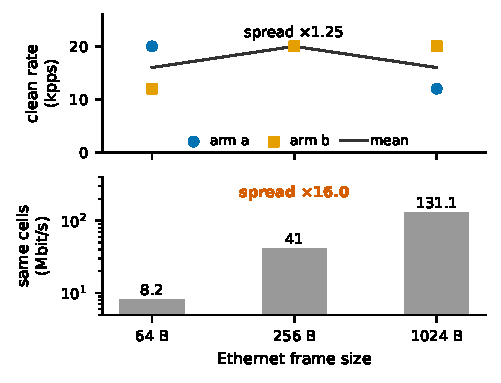
\includegraphics[width=.8\linewidth]{figs/fig1_unit_ambiguity}
\caption{The same six clean-rate cells, twice: packets per second are
near-flat ($\times1.25$, within $\pm$1 ladder rung) while the identical data
span $\times16.0$ as bit rate.}
\label{fig:unit}
\end{figure}

\textbf{(3) Flows.} With all $n$ flows pinned to one path class (so
flows/switch $=$ flows/link $=n$ by construction), the per-flow highest clean
rate falls monotonically in each of two independent arms, cells agreeing
within one ladder rung (Fig.~\ref{fig:flows}). The aggregate is an arithmetic
consequence; we report no ratio --- an earlier ``collapse factor'' divided a
clean threshold by a saturation knee, two different quantities, and was
withdrawn. Whether a production-grade datapath declines at all is an open
control we have not yet run on the same ladder.

\begin{figure}[t]
\centering

\includegraphics[width=.8\linewidth]{figs/fig2_perflow_monotone}
\caption{Per-flow highest clean rate vs.\ flow count: two independent arms,
each monotone. Gridlines are the ladder's rungs --- adjacent rungs are the
instrument's resolution.}
\label{fig:flows}
\end{figure}

\section{What limited our measurements}

For calibration: bmv2's documentation reports ${\sim}80$\,kpps for
\texttt{simple\_router.p4} on a dedicated cloud instance, two hosts, one
switch \cite{bmv2perf}. Our fast build reaches 16--20\,kpps --- 4--5$\times$
lower --- under a heavier P4 program, ten co-resident switches, veth links,
and a live control plane. We state this because it is exactly the comparison
the surveyed papers make impossible for their own numbers.

The same threat dominated all three experiments: \emph{our own instrument's
ceiling masquerading as the system's}. It happened twice (a flow-count
ladder's top rung briefly taken for the switch's ceiling; a build-ratio ladder
ending below the fast build's ability, censoring the numerator) and was
blocked once, by the registered sender gate. Both corrections moved
\emph{away} from the more publishable answer. None of the 12 measuring papers
reports a \emph{check} of what limited its own measurement --- three attribute
discrepancies after the fact, none measures the bound --- the same disease as
Mbps-without-size, in a second form.

\textbf{Scope.} bmv2 is a functional reference model; its own documentation
states it ``is not meant to be a production-grade software switch''
\cite{bmv2repo}. We do not report it as a performance target --- we report
that its published numbers cannot be compared. All measurements come from one
14-core host (Intel Core Ultra~5 125U, Linux 7.0.0-30-generic; no CPU pinning,
no fixed frequency), Mininet veth links (the size and flow experiments cross
two switches, h1$\to$h65; the build experiment one hop), one P4 program, one
behavioral-model commit (\texttt{f0b7d201}), predominantly UDP. \emph{The ratios do not transfer} to
another machine, another P4 program, or hardware targets, and say nothing
about P4 the language --- the same program on T4P4S reaches 2.3--2.6\,Gbps
\cite{kumazoe2023icncc}; what is slow is bmv2 as built for debugging. What
transfers is the structure: a variable this large, unreported, makes
comparison impossible.

\section{Takeaway}

\textbf{Why this matters beyond bmv2.} A large body of P4 work reports
speedups against a bmv2 baseline, and none of the 12 surveyed papers states
how its bmv2 was built --- so no reader can tell whether a reported speedup is
the mechanism's or the compiler's. On this machine that confound is worth
$8\times$: large enough to exceed many published gains outright. Nobody
compiles a functional model for speed; that is what makes it a dangerous
baseline, and why the build line must be reported. We therefore propose a
four-line provenance minimum for any software-switch number:
(1)~\textbf{build} --- flags and commit, e.g.\ ``\texttt{-O0 -g}, logging on,
\texttt{f0b7d201}''; (2)~\textbf{unit} --- pps with the frame size, or Mbps
with the size stated; (3)~\textbf{placement} --- flows per switch and per
link; (4)~\textbf{limit} --- what stopped the measurement: the system, or the
instrument.

\bibliographystyle{ACM-Reference-Format}
\bibliography{refs}

\end{document}
